\documentclass[logo,reportComp]{thesis}
\usepackage[cpp,pseudo]{mypackage}

\usetikzlibrary{automata,backgrounds,fit,shapes,positioning}

\tikzset{->, % makes the edges directed
>=stealth, % makes the arrow heads bold
node distance=2.5cm, % specifies the minimum distance between two nodes. Change if necessary.
every state/.style={thick, fill=gray!10}, % sets the properties for each 'state' node
}

\title{编译原理作业二}
\subtitle{}
\school{数据科学与计算机学院}
\author{陈鸿峥}
\classname{17大数据与人工智能}
\stunum{17341015}
\headercontext{编译原理作业}

% Apr 28 -> May 6

\begin{document}

\maketitle

\begin{question}
考虑以下NFA:
\begin{center}
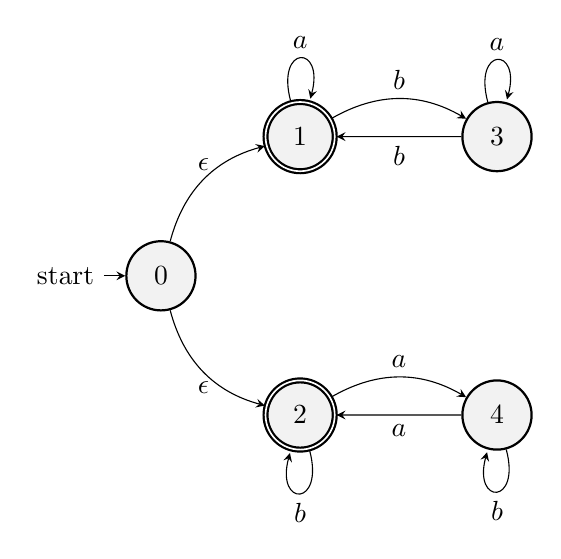
\begin{tikzpicture}[scale=0.6]
\node[state, initial] (0) {0};
\node[state, accepting, above right of=0] (1) {1};
\node[state, right of=1] (3) {3};
\node[state, accepting, below right of=0] (2) {2};
\node[state, right of=2] (4) {4};
\draw (0) edge[bend left, above] node{$\epsilon$} (1)
(0) edge[bend right, below] node{$\epsilon$} (2)
(1) edge[loop above] node{$a$} (1)
(2) edge[loop below] node{$b$} (2)
(1) edge[bend left, above] node{$b$} (3)
(3) edge[below] node{$b$} (1)
(3) edge[loop above] node{$a$} (3)
(2) edge[bend left, above] node{$a$} (4)
(4) edge[below] node{$a$} (2)
(4) edge[loop below] node{$b$} (4);
\end{tikzpicture}
\end{center}
\begin{enumerate}
	\item 这一NFA接受什么语言(用自然语言描述)?
	\item 构造接受同一语言的DFA.
\end{enumerate}
\end{question}
\begin{answer}
\begin{enumerate}
	\item 含有偶数个$a$或偶数个$b$的由$a$、$b$构成的字符串
	\item 由subset construction算法构造如下
\begin{center}
\begin{tabular}{|l|l|l|l|}\hline
NFA & DFA & $a$ & $b$\\\hline
$\{0,\underline{1,2}\}$ & $A$ & $\{1,4\}$ & $\{2,3\}$\\\hline
$\{\underline{1},4\}$ & $B$ & $\{1,2\}$ & $\{3,4\}$\\\hline
$\{\underline{2},3\}$ & $C$ & $\{3,4\}$ & $\{1,2\}$\\\hline
$\{\underline{1,2}\}$ & $D$ & $\{1,4\}$ & $\{2,3\}$\\\hline
$\{3,4\}$ & $E$ & $\{2,3\}$ & $\{1,4\}$\\\hline
\end{tabular}
\end{center}
\begin{center}
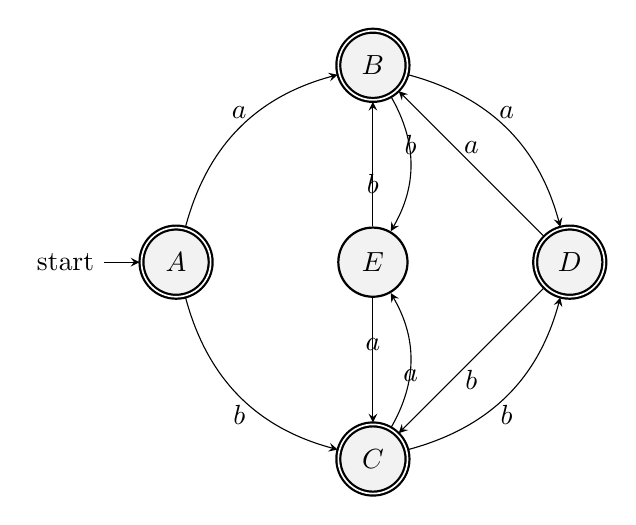
\begin{tikzpicture}
\node[state] (4) {$E$};
\node[state, accepting, initial, left of=4] (0) {$A$};
\node[state, accepting, above of=4] (1) {$B$};
\node[state, accepting, below of=4] (2) {$C$};
\node[state, accepting, right of=4] (3) {$D$};
\draw (0) edge[bend left, above] node{$a$} (1)
(0) edge[bend right, below] node{$b$} (2)
(1) edge[bend left, above] node{$a$} (3)
(1) edge[bend left, above] node{$b$} (4)
(2) edge[bend right, below] node{$a$} (4)
(2) edge[bend right, below] node{$b$} (3)
(3) edge[above] node{$a$} (1)
(3) edge[below] node{$b$} (2)
(4) edge[above] node{$a$} (2)
(4) edge[below] node{$b$} (1);
\end{tikzpicture}
\end{center}
\end{enumerate}
\end{answer}

\begin{question}
正则语言补运算
\begin{enumerate}
	\item 画出一个DFA,该DFA恰好识别所有含有$011$子串的二进制串.
	\item 画出一个DFA,该DFA恰好识别所有不含$011$子串的二进制串. 
	\item 再证明:对任一正则表达式$R$,一定存在另一正则表达式$R'$,使得$L(R')$是$L(R)$的补集.
\end{enumerate}
\end{question}
\begin{answer}
\begin{enumerate}
	\item 如下
\begin{center}
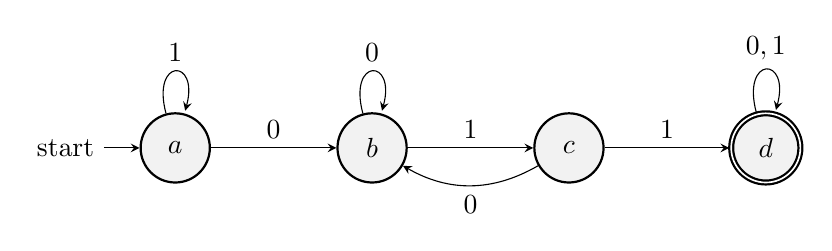
\begin{tikzpicture}
\node[state, initial] (0) {$a$};
\node[state, right of=0] (1) {$b$};
\node[state, right of=1] (2) {$c$};
\node[state, accepting, right of=2] (3) {$d$};
\draw (0) edge[above] node{$0$} (1)
(1) edge[above] node{$1$} (2)
(2) edge[above] node{$1$} (3)
(0) edge[loop above] node{$1$} (0)
(1) edge[loop above] node{$0$} (1)
(2) edge[bend left, below] node{$0$} (1)
(3) edge[loop above] node{$0,1$} (3);
\end{tikzpicture}
\end{center}
	\item 如下
\begin{center}
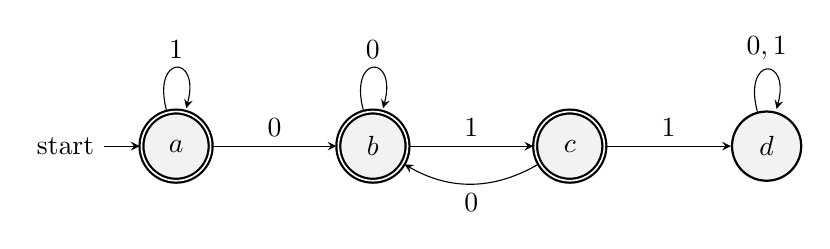
\begin{tikzpicture}
\node[state, accepting, initial] (0) {$a$};
\node[state, accepting, right of=0] (1) {$b$};
\node[state, accepting, right of=1] (2) {$c$};
\node[state, right of=2] (3) {$d$};
\draw (0) edge[above] node{$0$} (1)
(1) edge[above] node{$1$} (2)
(2) edge[above] node{$1$} (3)
(0) edge[loop above] node{$1$} (0)
(1) edge[loop above] node{$0$} (1)
(2) edge[bend left, below] node{$0$} (1)
(3) edge[loop above] node{$0,1$} (3);
\end{tikzpicture}
\end{center}
	\item 由正则表达式与DFA的等价性,对于正则表达式$R$,必然存在DFA $M$可以识别$L(R)$,那么将$M$中的接受状态改为非接受状态,将非接受状态改为接收状态,得到新的DFA $M'$可以识别$L(R)$的补集,进而存在$M'$对应的正则表达式$R'$,使得$L(R')$是$L(R)$的补集.
\end{enumerate}
\end{answer}

\begin{question}
设有一门小小语言仅含\texttt{z}、\texttt{o}、\texttt{/}(斜杠)3个符号,该语言中的一个注释以一个\texttt{/o}为开始标记,以此后出现的第一个\texttt{o/}为结束标记.
\begin{enumerate}
	\item 请给出单个正则表达式,它仅与一个完整的注释匹配,除此之外不匹配任何其他串。
	书写正则表达式时,要求仅使用最基本的正则表达式算子($\epsilon$,$|$,${}^*$,$+$,$?$).
	\item 给出识别上述正则表达式所定义语言的确定有限自动机(DFA).
	你可根据问题直接构造DFA,不必运用机械的算法从上一小题的正则表达式转换得到DFA.
\end{enumerate}
\end{question}
\begin{answer}
\begin{enumerate}
	\item $/o\ (o^*z\mid/)^*\ o+/$
	\item 如下
\begin{center}
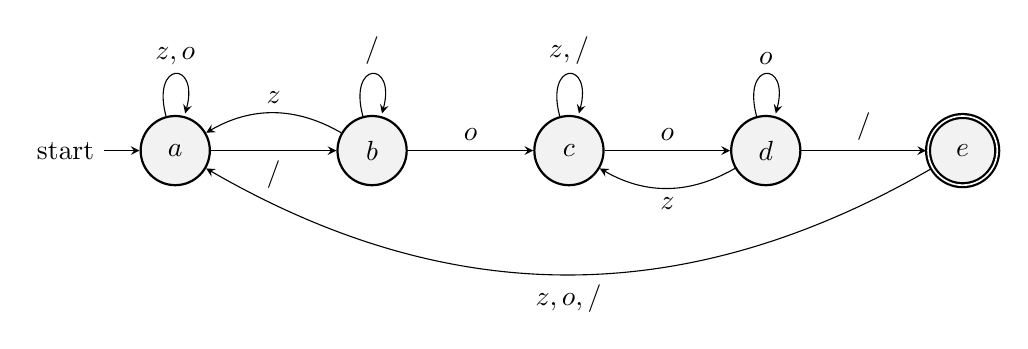
\begin{tikzpicture}
\node[state, initial] (0) {$a$};
\node[state, right of=0] (1) {$b$};
\node[state, right of=1] (2) {$c$};
\node[state, right of=2] (3) {$d$};
\node[state, accepting, right of=3] (4) {$e$};
\draw (0) edge[below] node{$/$} (1)
(1) edge[above] node{$o$} (2)
(2) edge[above] node{$o$} (3)
(3) edge[above] node{$/$} (4)
(0) edge[loop above] node{$z,o$} (0)
(1) edge[loop above] node{$/$} (1)
(1) edge[bend right, above] node{$z$} (0)
(2) edge[loop above] node{$z,/$} (2)
(3) edge[loop above] node{$o$} (3)
(3) edge[bend left, below] node{$z$} (2)
(4) edge[bend left, below] node{$z,o,/$} (0);
\end{tikzpicture}
\end{center}
\end{enumerate}
\end{answer}

\end{document}